%\chapter{控制分配问题}
\chapter{涵道风扇式无人机建模}
%
本章首先针对如图\ref{DFUAV}所示的单涵道风扇式无人机进行建模,然后简单介绍如图\ref{TDFUAV}所示的双涵道,及其在悬停点附近的气动力和力矩的数学模型。在建模过程中将飞行器视为刚体,利用常规的飞行器建模方法,推导其六自由度运动方程。该方程描述了所研究的涵道风扇式无人机的飞行动力学,借助MATLAB$^\circledR$/Simulink$^\circledR$软件实时求解该方程,可以模拟飞行器对给定输入的响应。运动方程的数学表达式是根据特定的坐标系建立的,本章首先介绍建模所需的坐标系,将飞行器的平移运动和旋转运动参数化。其次,根据牛顿-欧拉法建立描述飞行器行为的微分方程。最后,分别对单、双涵道,分析所受的气动力和力矩。
\begin{figure}[htbp]
	\centering
	\begin{minipage}[c]{0.5\textwidth}
		\centering
		\includegraphics[scale=1]{Fig/DFUAV_f31.png}
	\end{minipage}%
	\begin{minipage}[c]{0.5\textwidth}
		\centering
		\includegraphics[scale=0.41]{Fig/TwinductedfanUAV.jpg}
	\end{minipage}\\[1pt]
	\begin{minipage}[t]{.5\textwidth}
		\caption{\label{DFUAV}单涵道风扇式无人机}
	\end{minipage}%
	\begin{minipage}[t]{.5\textwidth}
		\caption{\label{TDFUAV}双涵道风扇式无人机}
	\end{minipage}%
\end{figure}
\section{坐标系定义及运动方程}
\subsection{坐标系定义}
涵道风扇式无人机的六自由度运动包括平移和旋转运动,为方便描述,引入如下坐标系:
\begin{enumerate}
	\item	地理坐标系${\bm{X}_n}{\bm{Y}_n}{\bm{Z}_n}$
	
	地理坐标系的原点$ \bm{O} $定义为无人机的起飞点,与起飞点固连,在导航中将其作为惯性参考系。其 $ \bm{O}\bm{X}_n $ 轴指向当地的正北方向,$ \bm{O}\bm{Y}_n$轴指向正东方向,$ \bm{O}\bm{Z}_n $轴垂直地面向下。又称“北东地(NED)”坐标系。
	 
	\item	机体坐标系${\bm{X}_b}{\bm{Y}_b}{\bm{Z}_b}$
	
	机体坐标系的原点$ \bm{O} $与无人机的重心固连。其 $ \bm{O}\bm{X}_b $ 轴指向认为定义的机头方向, $ \bm{O}\bm{Y}_b  $轴垂直于机头方向所在的机体对称平面指向机体右侧,$ \bm{O}\bm{Z}_b $轴则取为和$ \bm{O}\bm{X}_b $轴、 $ \bm{O}\bm{Y}_b  $轴成右手系的方向 。
\end{enumerate}	

以单涵道为例,地理坐标系${\bm{X}_n}{\bm{Y}_n}{\bm{Z}_n}$和机体坐标系${\bm{X}_b}{\bm{Y}_b}{\bm{Z}_b}$如图\ref{fig_NED_B}所示。无人机重心相对NED系的位置矢量在NED系中的投影记为$\bm{P} $,机体重心的相对NED系的速度矢量在NED系中的投影记为$ \bm{V}_n$ ,机体重心的相对NED系的速度矢量在机体系中的投影记为$ \bm{V}_b=[u \quad v \quad w]^\top $。
%=[V_x \quad V_y \quad V_z]^\top	
	
旋转运动可以用四元数、欧拉角、旋转矩阵等方法描述,本文主要使用欧拉角描述无人机的机体系相对NED系的旋转。旋转运动和坐标系的原点无关,在求取欧拉角时可令NED系原点和机体系原点重合,以单涵道为例,如图\ref{fig_euler}所示。机体坐标系相对NED坐标系旋转的角速度矢量在机体系中的投影记为$ \bm{\omega}= [p \quad q \quad r]^\top $。欧拉角定义为:NED坐标系绕$ \bm{Z}_n $轴旋转偏航角$ \psi $,再绕当前$ \bm{Y}^{'}_n$轴旋转俯仰角$ \theta $,最后绕当前$ \bm{X}^{'}_n$轴旋转滚转角$ \varphi $。由欧拉角表示的机体坐标系到地面坐标系的旋转矩阵记为$ \bm{R}^n_b $,有$ ({\bm{R}^n_b})^T=\bm{R}^b_n $。记$ \bm{R}^n_b $为$ \bm{R}  $,并记正弦函数为$ S $,余弦函数为$ C $,则有
\begin{align}
\bm{R}=\begin{bmatrix}
C \psi C \theta & -S \psi C \varphi+C \psi S \theta S \varphi & S \psi S \varphi+C \psi S \theta C \varphi \\
S \psi C \theta & C \psi C \varphi+S \psi S \theta S \varphi & -C \psi S \varphi+S \psi S \theta C \varphi \\
-S \theta & C \theta S \varphi & C \theta C \varphi
\end{bmatrix}
\end{align}
%按$\bm{XYZ}$的顺序定义的欧拉角$\varphi$、$\theta$、$\psi$如图\ref{fig_euler}所示,坐标系原点为无人机重心。记绕机体坐标系转动的角速度为$\bm{\omega}$。
\begin{figure}[htbp]
	\centering
	\begin{minipage}[c]{0.5\textwidth}
		\centering
		\includegraphics[scale=1]{Fig/Fig_NED_B.pdf}
	\end{minipage}%
	\begin{minipage}[c]{0.5\textwidth}
		\centering
		\includegraphics[scale=1]{Fig/Fig_euler.pdf}
	\end{minipage}\\[1pt]
	\begin{minipage}[t]{.5\textwidth}
		\caption{\label{fig_NED_B}地面坐标系及机体坐标系}
	\end{minipage}%
	\begin{minipage}[t]{.5\textwidth}
		\caption{\label{fig_euler}欧拉角的定义}
	\end{minipage}%
\end{figure}
%\section{运动方程}
通常推导无人机的运动方程时假定它是一个刚体,而地理坐标系是惯性系(地球是平的假定)。通常无人机在低速度和短时间内的机动,其中由于地球的旋转产生的向心角速度,科里奥利加速度和切向加速度的影响可以忽略的,因此平面地球假设是合理的。
\subsection{运动学方程}
六自由度刚体的运动学方程由质点的运动学方程和欧拉运动学方程描述,分别为
\begin{align}
\dot{\bm{P}}=\bm{V}_n	\label{eq_k_pos}
\end{align}
\begin{align}
\begin{bmatrix}
\dot{\varphi} \\
\dot{\theta} \\
\dot{\psi}
\end{bmatrix}=
\begin{bmatrix}
1 & \sin \varphi \tan \theta & \cos \varphi \tan \theta \\
0 & \cos \varphi & -\sin \varphi \\
0 & \dfrac{\sin \varphi}{\cos \theta} & \dfrac{\cos \varphi}{\cos \theta}
\end{bmatrix}
\begin{bmatrix}
p \\
q \\
r
\end{bmatrix}	\label{eq_k_euler}
\end{align}
为了方便后续的推导,这里不加证明地给出旋转矩阵导数的表达式
\begin{align}
\dot{\bm{R}}=\bm{R}[\bm{\omega}]_{\times} \label{eq_drot}
\end{align}
其中叉乘算子$ [\bm{\omega}]_{\times} $的表达式为
\begin{align}
[\bm{\omega}]_{\times}=
\begin{bmatrix}
0 & -r & q \\
r & 0 & -p \\
-q & p & 0
\end{bmatrix} 
\end{align}
\subsection{动力学方程}
无人机的位置动力学方程及其旋转动力学方程通常分别由动量定理和角动量定理推出。另外,无人机所受的除重力外其他力的矢量和、合力矩在机体系中的表示比较方便,而动量定理和角动量定理只有在惯性系(NED系)中才成立。因此在非惯性系(机体系)中表示的动力学方程需要通过旋转变换得到。对于位置动力学方程,在NED系中由动量定理(或由牛顿第二定律),有
\begin{align}
\dfrac{d(m\bm{V}_n)}{d t}=m \dot{\bm{V}}_n=\bm{R}\bm{F}+\bm{G}	\label{eq_d_pos}
\end{align}
其中$ \bm{G}=mg $为无人机所受重力,$ \bm{F} $为除重力外其他力的矢量和,在本文中主要指所有气动力的矢量和。很多文献还会在非惯性系中表示该方程,这里简单给出推导。由速度矢量的坐标变换关系
\begin{align}
\bm{V}_n=\bm{R}\bm{V}_b
\end{align}
两边同时求导得
\begin{align}
\dot{\bm{V}_n}=\dot{\bm{R}}\bm{V}_b+\bm{R}\dot{\bm{V}_b}=\bm{R}[\bm{\omega}]_{\times}\bm{V}_b+\bm{R}\dot{\bm{V}_b}
\end{align}
代入式\eqref{eq_d_pos}有
\begin{align}
m(\bm{\omega} \times \bm{V}_b+\dot{\bm{V}_b})=\bm{F}+\bm{R}^T\bm{G}
\end{align}

在惯性系NED系中应用角动量定理稍有不同,惯性张量在NED中的表示$ {\bm{I}}^{'} $将是一个变量,而再机体系中的表示是一个常量,因此旋转动力学方程一般都是在机体系中表示。记NED系中角动量为$ {\bm{L}}^{'} $,机体坐标系相对NED坐标系旋转的角速度矢量在NED系中的投影为$ {\bm{\omega}}^{'} $,则NED系中的角动量表示为
\begin{align}
{\bm{L}}^{'} ={\bm{I}}^{'} {\bm{\omega}}^{'}
\end{align}
由旋转变换关系$ {\bm{\omega}}^{'}=\bm{R} \bm{\omega} $,得
\begin{align}
{\bm{L}}^{'}=\bm{R} \bm{L}=\bm{R} \bm{I} \bm{\omega}=\bm{R} \bm{I} \bm{R}^T {\bm{\omega}}^{'}
\end{align}
故有$ \bm{R} \bm{I} \bm{R}^T= {\bm{I}}^{'}  $。根据角动量定理,有
\begin{align}
\dfrac{d({\bm{I}}^{'} {\bm{\omega}}^{'})}{d t}={\bm{M}}^{'}
\end{align}
其中$ {\bm{M}}^{'} $为NED系中表示的合力矩。应用坐标变换,上式变为
\begin{align}
\dfrac{d(\bm{R} \bm{I} \bm{R}^T \bm{R} \bm{\omega})}{d t} = \bm{R} \bm{M} \label{eq_angular_momentum}
\end{align}
其中$ \bm{M} $为在机体系中表示的合力矩。结合式\eqref{eq_drot}对式\eqref{eq_angular_momentum}等式左边化简,得
\begin{align}
\dfrac{d(\bm{R} \bm{I} \bm{R}^T \bm{R} \bm{\omega})}{d t}=\dfrac{d(\bm{R} \bm{I} \bm{\omega})}{d t}=\dot{\bm{R}} \bm{I} \bm{\omega} + \bm{R} \bm{I} \dot{\bm{\omega}} = \bm{R}[\bm{\omega}]_{\times} \bm{I} \bm{\omega} + \bm{R} \bm{I} \dot{\bm{\omega}}
\end{align}
联立式\eqref{eq_angular_momentum},得欧拉动力学方程
\begin{align}
\dot{\bm{\omega}} = \bm{I}^{-1}(\bm{M}-\bm{\omega} \times \bm{I} \bm{\omega}) \label{eq_d_euler} 
\end{align}
将式\eqref{eq_k_pos}、式\eqref{eq_k_euler}、式\eqref{eq_d_pos}、式\eqref{eq_d_euler}整理合并,得涵道无人机的非线性模型\cite{Pflimlin_2007a,Zhao_2015}
\begin{equation}
\left\lbrace 
\begin{aligned}
\dot{\bm{P}} & = \bm{V}_n	\\
\dot{\bm{V}}_n & =\dfrac{1}{m}(\bm{R}\bm{F}+\bm{G})	\\
\begin{bmatrix}
\dot{\varphi} \\
\dot{\theta} \\
\dot{\psi}
\end{bmatrix} & =
\begin{bmatrix}
1 & \sin \varphi \tan \theta & \cos \varphi \tan \theta \\
0 & \cos \varphi & -\sin \varphi \\
0 & \dfrac{\sin \varphi}{\cos \theta} & \dfrac{\cos \varphi}{\cos \theta}
\end{bmatrix}
\begin{bmatrix}
p \\
q \\
r
\end{bmatrix}	\\
\dot{\bm{\omega}} & = \bm{I}^{-1}(\bm{M}-\bm{\omega} \times \bm{I} \bm{\omega})
\end{aligned}
\right. 		\label{eq_nonlinear_model}
\end{equation}
其中作用于无人机的力$ \bm{F} $和力矩$ \bm{M} $在机体系上的投影。上述方程对于单/双涵道来说是一样的,唯一不同的是作用于机体的力$ \bm{F} $和力矩$ \bm{M} $的具体表达式不相同。尽管如此,单/双涵道仍有很多相似之处。单/双涵道的气动力和气动力矩分析将在后两节介绍。
%式中:$\bm{\Gamma } = \bm{\Gamma} _{cs} + \bm{\Gamma} _{ext}$。$\bm{\Gamma} _{cs}$为操纵面产生的驱动力矩,$\bm{\Gamma} _{ext}$为其他力矩\cite{Pflimlin_2007a},$\bm{I}=\operatorname{diag}\left(I_{x}, I_{y}, I_{z}\right)$为惯性张量。
\section{单涵道动力学分析}
%创建了GTSpy模型,用于仿真以验证适当的控制器行为。 以下各节详细介绍了此模型的公式,并在附录中列出了GTSpy的数值。 由于仿真的主要重点是控制器验证,因此对作用在车辆上的主要力和力矩建模至关重要。 只要这些力和力矩表现出适当的功能依赖性并且具有正确的意义和数量级,那么准确预测这些力和力矩就对该模型而言至关重要。 因此,在某些方面进行了简化的假设,因为所需的保真度不能证明增加的复杂性。
%基本动力学方程为:
%\begin{align}
%\dot{\bm{v}} &=\dfrac{F}{m}	\\
%\dot{\bm{\omega}} &=\bm{I}^{-1}(\bm{M}-\bm{\omega} \times \bm{I} \bm{\omega}) \label{eq_d_eulera}
%\end{align}
%其中$ p \in \mathbb{R}^3 $代表位置矢量,$v \in \mathbb{R}^3 $是速度矢量,$ q \in \mathbb{R}^4 $是四元数矢量,$ \omega \in \mathbb{R}^3 $表示角速度矢量。 车辆质量由$ m $表示,$ q_i $代表四个
%四元数向量的分量,$ \bm{I} $是车辆惯性矩阵,$ \bm{F} $和$ \bm{M} $项表示
%作用在车辆上的外力和力矩矢量。 力和力矩矢量可以表示为:
在单涵道中,力$ \bm{F} $和力矩$ \bm{M} $可以表示为
\begin{align}
\bm{F} &=\bm{F}_{a}+\bm{F}_{r}+\bm{F}_{d}+\bm{F}_{c} \\
\bm{M} &=\bm{M}_{a}+\bm{M}_{r}+\bm{M}_{d}+\bm{M}_{c}+\bm{M}_{g}+\bm{M}_{a f}
\end{align}
其中$ \bm{F}_a $和$ \bm{M}_{a} $表示由机身空气阻力产生的力和力矩,$ \bm{F}_{r} $和$ \bm{M}_{r} $表示涵道内部的风扇产生的升力和力矩,$ \bm{F}_{d} $和$ \bm{M}_{d} $表示涵道翼型产生的力和力矩,$ \bm{F}_{c} $和$ \bm{M}_{c} $表示涵道底部的控制舵产生的力和力矩,$ \bm{M}_{g} $为陀螺力矩,$ \bm{M}_{a f} $为固定气动面扭矩。下面将逐一分析各个力和力矩的表达式。
\subsection{机身动力学}
机身气动阻力及其产生的力矩可以写为\cite{Johnson_2005}:
\begin{align}
\bm{F}_{{a}} &=-\dfrac{1}{2} \rho\begin{bmatrix}
C_{D, x} A_x u\left|u\right| \\
C_{D, y}  A_y v\left|v\right| \\
C_{D, z}  A_z w\left|w\right|
\end{bmatrix}  	\label{eq_F_a}
\end{align}
\begin{align}
\bm{M}_{{a}} &=\dfrac{1}{2} \rho
\begin{bmatrix}
C_{D, y} A_y v\left|v\right| \\
-C_{D, x} A_x u\left|u\right| \\
0
\end{bmatrix} l_{a }	\label{M_aero}
\end{align}
其中,$ \rho $代表空气密度,$ C_{D,x} $、$ C_{D,y} $、$ C_{D,z} $分别表示无人机沿机体轴$ x $,$ y $,$ z $方向的阻力系数,$A_x $、$ A_y $、$ A_z $分别表示无人机沿机体轴$ x $,$ y $,$ z $方向的截面面积,$ l_{a} $为机身气动阻力作用点与重心之间的距离。
\subsection{涵道风扇动力学}
与直升机相似,假设流动为管流,建立涵道风扇轴流状态的管流模型\cite{Liu_2006}。气体在无穷远处速度为$ V_c $,经过风扇桨盘时加速至$ V_c+V_i $,最终以$ V_c+V_2 $形成尾迹。如图\ref{fig_Duct_dynamic}所示。
\begin{figure}[htbp]
	\centering
	\includegraphics[scale=1]{Fig/Fig_Duct_dynamic.pdf}
	\caption{\label{fig_Duct_dynamic}轴流状态的空气动力学}
\end{figure}

与孤立旋翼不同,涵道体上也产生拉力$ T_d $,设风扇拉力为$ T_p $,总拉力为$ T_a $,并定义涵道拉力分配系数$ q_a $为:
\begin{align}
q_a=T_d/T_a=T_d/(T_d+T_p )
\end{align}
忽略桨盘厚度,则认为气体经过桨盘时发生压强突变,而速度则是均匀增加。设桨盘上表面压强为$ p_U $,下表面压强为$ p_L $。则桨盘上下表面处的气体速度均为$ V_c+V_i $。在桨盘上方和下方管流分别应用Bernouli方程
\begin{align}
p_\infty+1/2 ρV_c^2=p_U+1/2 ρ(V_c+V_i )^2	\label{eq_q}
\end{align}
\begin{align}
p_L+1/2 ρ(V_c+V_i )^2=p_\infty+1/2 ρ(V_c+V_2 )^2	
\end{align}
设桨盘面积为S,则风扇拉力由风扇桨盘上下压差产生:
\begin{align}
T_p=S(p_L-p_U )=ρS(V_c+V_2/2) V_2	\label{eq_T_p}
\end{align}
另一方面,从气体动量角度分析,涵道风扇对气流的总作用力应等于单位时间内通过桨盘气体动量的增量,即:
\begin{align}
T_a=T_d+T_p=\dot{m}_{air} V_2=ρS(V_c+V_i ) V_2	\label{eq_T_a}
\end{align}
由式\eqref{eq_q}、\eqref{eq_T_p}、\eqref{eq_T_a}可得:
\begin{align}
T_a=q_aT+T_p= q_aρS(V_c+V_i ) V_2+ ρS(V_c+V_2/2) V_2	\label{eq_T_a1}
\end{align}
比较式\eqref{eq_T_a}、\eqref{eq_T_a1}可得
\begin{align}
V_2=2[(1-q_a) V_i-q_aV_c ]	\label{eq_V_2}
\end{align}
将\eqref{eq_V_2}代入\eqref{eq_T_a1}中可得:
\begin{align}
(1-q_a) V_i^2+(1-2q_a) V_c V_i-(T_a/2ρS+q_aV_c^2 )=0	\label{eq_function}
\end{align}
视\eqref{eq_function}为关于$ V_i $的一元二次方程,取正根可解得:
\begin{align}
V_{i}=-\frac{(1-2 q_a) V_{c}}{2(1-q_a)}+\sqrt{\left(\dfrac{V_{c}}{2(1-q_a)}\right)^{2}+\dfrac{T_a}{2 \rho S(1-q_a)}} \label{eq_Vi}	\\
V_{c}+V_{i}=\dfrac{V_{c}}{2(1-q_a)}+\sqrt{\left(\dfrac{V_{c}}{2(1-q_a)}\right)^{2}+\frac{T_a}{2 \rho S(1-q_a)}}	\label{eq_Vi_Vc}
\end{align}
桨盘处气流诱导速度$ V_i $及气流速度$ V_c+V_i $在后续的空气动力学分析中极其重要,包括控制舵面上的气动力、飞行器前飞时的动量阻力与附加阻力等核心气动力的计算。

式\eqref{eq_Vi_Vc}和式\eqref{eq_Vi}表明了一种特殊情况,当$ V_c=-V_{cr} $,满足:
\begin{align}
-V_{cr}+V_i=0
\end{align}
其中$ V_{cr} $为飞行器理想自转下降状态下的下降速率,该速率下风扇消耗功率为0,飞行器能在无动力情况下实现安全着陆。当$ -V_c>V_{cr} $时,风扇桨盘处流场呈复杂涡流状态,管流模型不再适用,此时飞行器气动状态复杂且不稳定。在实际飞行中应控制下降/刹车速率,防止进入涡流状态。

涵道风扇的拉力$ T_p $解析式与风扇桨叶外形有关,不具有统一形式。但对一般涵道风扇,可由下式近似给出:
\begin{align}T_p = k_{\varpi} \varpi^{2}\end{align}
%+k_{v \varpi} V_{c} \varpi
%\begin{align}
%T_a=k_{\varpi} \varpi^{2}
%\end{align}
其中$ k_{\varpi} $为常系数。将上述方程迭代求解,可得作用于无人机的推力
\begin{align}
\bm{F}_{r}=\begin{bmatrix}
0\\0\\
-T_a
\end{bmatrix}
\end{align}
与拉力$ T_a $类似,涵道风扇产生的扭矩$ Q $的解析式与风扇桨叶外形有关,不具有统一形式,可由下式近似表示\cite{Stiltner_2012,Graf_2008}
\begin{align}
Q=d_{\varpi} { \varpi }^{2} 	\label{eq_Q}
%+d_{v \varpi} V_{c} \varpi
\end{align}
其中$ \varpi $为风扇转速,$ d_{\varpi}  $为常系数。涵道风扇仅在机体系$ \bm{Z}_B $轴产生扭矩,因而有
\begin{align}
\bm{M}_{r}=\begin{bmatrix}
0\\0\\
Q
\end{bmatrix}
\end{align}
\subsection{涵道动力学}
作用在涵道环形机翼上的气动力可以用升力-阻力模型来估算。 使用不可压缩的稳态流理论,简化围绕涵道的高度非稳态气流。 

取$ \mu $为环绕涵道的角度变量,以$ \hat{\bm{i}} $,$ \hat{\bm{j}} $为沿无人机机体系的$ x $轴和$ y $轴方向的单位矢量。 涵道机体系 $x $轴和$ y $轴构成的平面中径向单位矢量和气流流速矢量的径向分量可以表示为\cite{Johnson_2005}
\begin{align}\hat{\bm{e}}_{{r}}=\hat{\bm{i}} \cos \mu+\hat{\bm{j}} \sin \mu\end{align}
\begin{align}
\bm{V}_{{x y}}=-u \hat{\bm{i}}-v \hat{\bm{j}}	\label{flow_velocity_xy}
\end{align}
式\eqref{flow_velocity_xy}中的速度项表示无人机相对于空气的速度,因此使用负号表示气流相对于机体的速度。径向气流流速是环绕涵道的角度变量$ \mu $和空气流速在机体系$ z $轴分量的函数
\begin{align}\begin{array}{c}
V_{r}(\mu)=\bm{V}_{{xy}} \cdot \hat{\bm{e}}_{{r}}=-u \cos \mu-v \sin \mu \\
V_{z}(\mu)=V_{i}-w
\end{array}\end{align}
上式假设$ z $轴分量在涵道周围是恒定的。 涵道圆周上每个位置的动压力和迎角为
\begin{align}
\begin{array}{c}
q_{d}(\mu)=\dfrac{1}{2} \rho\left(V_{r}^{2}+V_{z}^{2}\right) \\
\alpha_{d}(\mu)=\tan ^{-1}\left(\dfrac{V_{r}}{V_{z}}\right)
\end{array}
\end{align}
围绕涵道的每单位展长的升力和阻力
\begin{align}l(\mu)=C_{l, d}(\alpha_d) q_{d} c_{d}, \quad d(\mu)=C_{d, d}(\alpha_d) q_{d} c_{d}\end{align}
其中$ C_{l, d}(\alpha_d) $是涵道翼型升力曲线,$ C_{d, d}(\alpha_d) $是涵道翼型阻力曲线,$ c_d $是涵道翼型弦长。 由于包括涵道的翼型是对称的,因此俯仰力矩可忽略。 每单位展长的升力和阻力的组成可表示为
\begin{align}
\begin{array}{cl}
l_{x}=l(\mu) \cos \alpha_d \cos \mu ,\quad d_{x}=d(\mu) \sin \alpha_d \cos \mu \\
l_{y}=l(\mu) \cos \alpha_d \sin \mu ,\quad d_{y}=d(\mu) \sin \alpha_d \sin \mu \\
l_{z}=-l(\mu) \sin \alpha_d ,\quad d_{z}=d(\mu) \cos \alpha_d
\end{array}
\end{align}
将上述各轴分量进行积分可得到各轴方向的升力和阻力, 以升力$ x $轴分量为例,有
\begin{align}
L_{x}=r \int_{0}^{2 \pi} l_{x} d \mu
\end{align}
涵道翼型的升力和阻力曲线可近似表示为\cite{Johnson_2005}
\begin{align}
C_{l, d}(\alpha_d)=\min \left(C_{l, \max }, \max \left(\dfrac{1}{2} C_{l_{\alpha}} \sin (2 \alpha_d), \quad C_{l, \min }\right)\right)
\end{align}
\begin{align}
C_{d, d}(\alpha_d)=C_{d, o }-C_{d, g } \cos (2 \alpha_d)
\end{align}
其中$ C_{l_{\alpha}} $表示风管翼型升力曲线斜率,$ C_{l, \min } $和$ C_{l, \max } $表示升力系数的极限,$ C_{d, o } $和$ C_{d, g } $为用于拟合阻力曲线的经验常数。 图将上式计算得到的升力和阻力曲线与雷诺数为80000的NACA 0015机翼的数据\cite{Sheldahl_1981}进行了比较。所研究的涵道无人机雷诺数远低于80000,估计升力曲线和实验升力曲线之间也存在一些差异,但未简单起见,仍采用该经验公式。
\begin{figure}[htbp]
	\centering
	\includegraphics[scale=1]{Fig/Fig_C_L.pdf}
	\caption{\label{Fig_C_L}升力系数}
\end{figure}
\begin{figure}[htbp]
	\centering
	\includegraphics[scale=1]{Fig/Fig_C_D.pdf}
	\caption{\label{Fig_C_D}阻力系数}
\end{figure}

在有侧风的情况下,涵道将改变来流的方向,以使其与涵道$ z $轴对齐。 这会使涵道受到反作用力,即动量阻力,从而使无人机迎风飞行。 动量阻力可表示为\cite{Fleming_2003}
\begin{align}\bm{F}_{{m}}=-V_{i} \rho \pi R^{2}\left[\begin{array}{c}
u \\
v \\
0
\end{array}\right]\end{align}
其中$ R $为风扇半径。当周围的空气被风扇吸入涵道内时,侧风还会在涵道的上边缘产生低压区。 从而使得唇缘上产生更大的升力,进而使无人机偏离侧风,产生的力矩可表示为\cite{Fleming_2003}
\begin{align}\bm{M}_{{l}}=\rho R C_{d u c t} \left[\begin{array}{r}
v\left|v\right| \\
-u\left|u\right| \\
0
\end{array}\right]\end{align}
其中$ C_{d u c t} $为常值比例系数。 对于侧风产生的力矩,上式只是近似值,假定了力矩与侧风引起的动压力成比例。 常值比例系数最早由文献\parencite{Fleming_2003}提供的实验数据估算得,可根据无人机实际飞行测试进行了调整。

综上所述,涵道产生的力和力矩可分别表示为
\begin{align}
\bm{F}_{{d}}=
\begin{bmatrix}
L_{x}+D_{x} \\
L_{y}+D_{y} \\
L_{z}+D_{z}
\end{bmatrix}
+\bm{F}_{{m}} 
\end{align}
\begin{align}
\bm{M}_{{d}}=
\begin{bmatrix}
L_{x} l_{d} \\
L_{y} l_{d} \\
0
\end{bmatrix}
+\bm{M}_{{l}}
\end{align}
其中$ l_{d} $代表无人机重心与涵道气动力作用点之间的距离。 
%在此模型中,忽略了由于拖曳力而产生的力矩。

%可以根据提升力分量计算出由导管引起的下洗角。 升力通常通过以下表达式与下洗角度相关:
%\begin{align}
%L=\dot{m}v\gamma
%\end{align}
%其中$ \dot{m} $和$ \gamma $代表质量流量和流速。 该公式产生沿$ x $和$ y $轴的下洗角的表达式:
%\begin{align}
%\gamma_{x}=\dfrac{L_{x}}{\rho_{\infty} \pi r^{2}\left[\left(v_{i}-v_{z}\right)^{2}+v_{x}^{2}\right]} \\
%\gamma_{y}=\dfrac{L_{y}}{\rho_{\infty} \pi r^{2}\left[\left(v_{i}-v_{z}\right)^{2}+v_{y}^{2}\right]}
%\end{align}
%在对管道空气动力学进行建模时,尤其是在需要更精确的性能评估时,可以使用另一种方法,即使用计算流体动力学来形成空气动力学系数的数据库,在仿真过程中可以访问该数据库以制定空气动力学力和力矩。 如果有这样的数据库,或者需要更高程度的空气动力学保真度,则可以替换上面给出的管道模型。
\subsection{操纵面动力学}
\begin{figure}[htbp]
	\centering
	\includegraphics[scale=1]{Fig/Fig3.pdf}
	\caption{\label{DFUAV_arm}单涵道力臂示意图}
\end{figure}
%\begin{figure}[htbp]
%	\centering
%	\begin{minipage}[c]{0.45\textwidth}
%		\centering
%%		\fbox{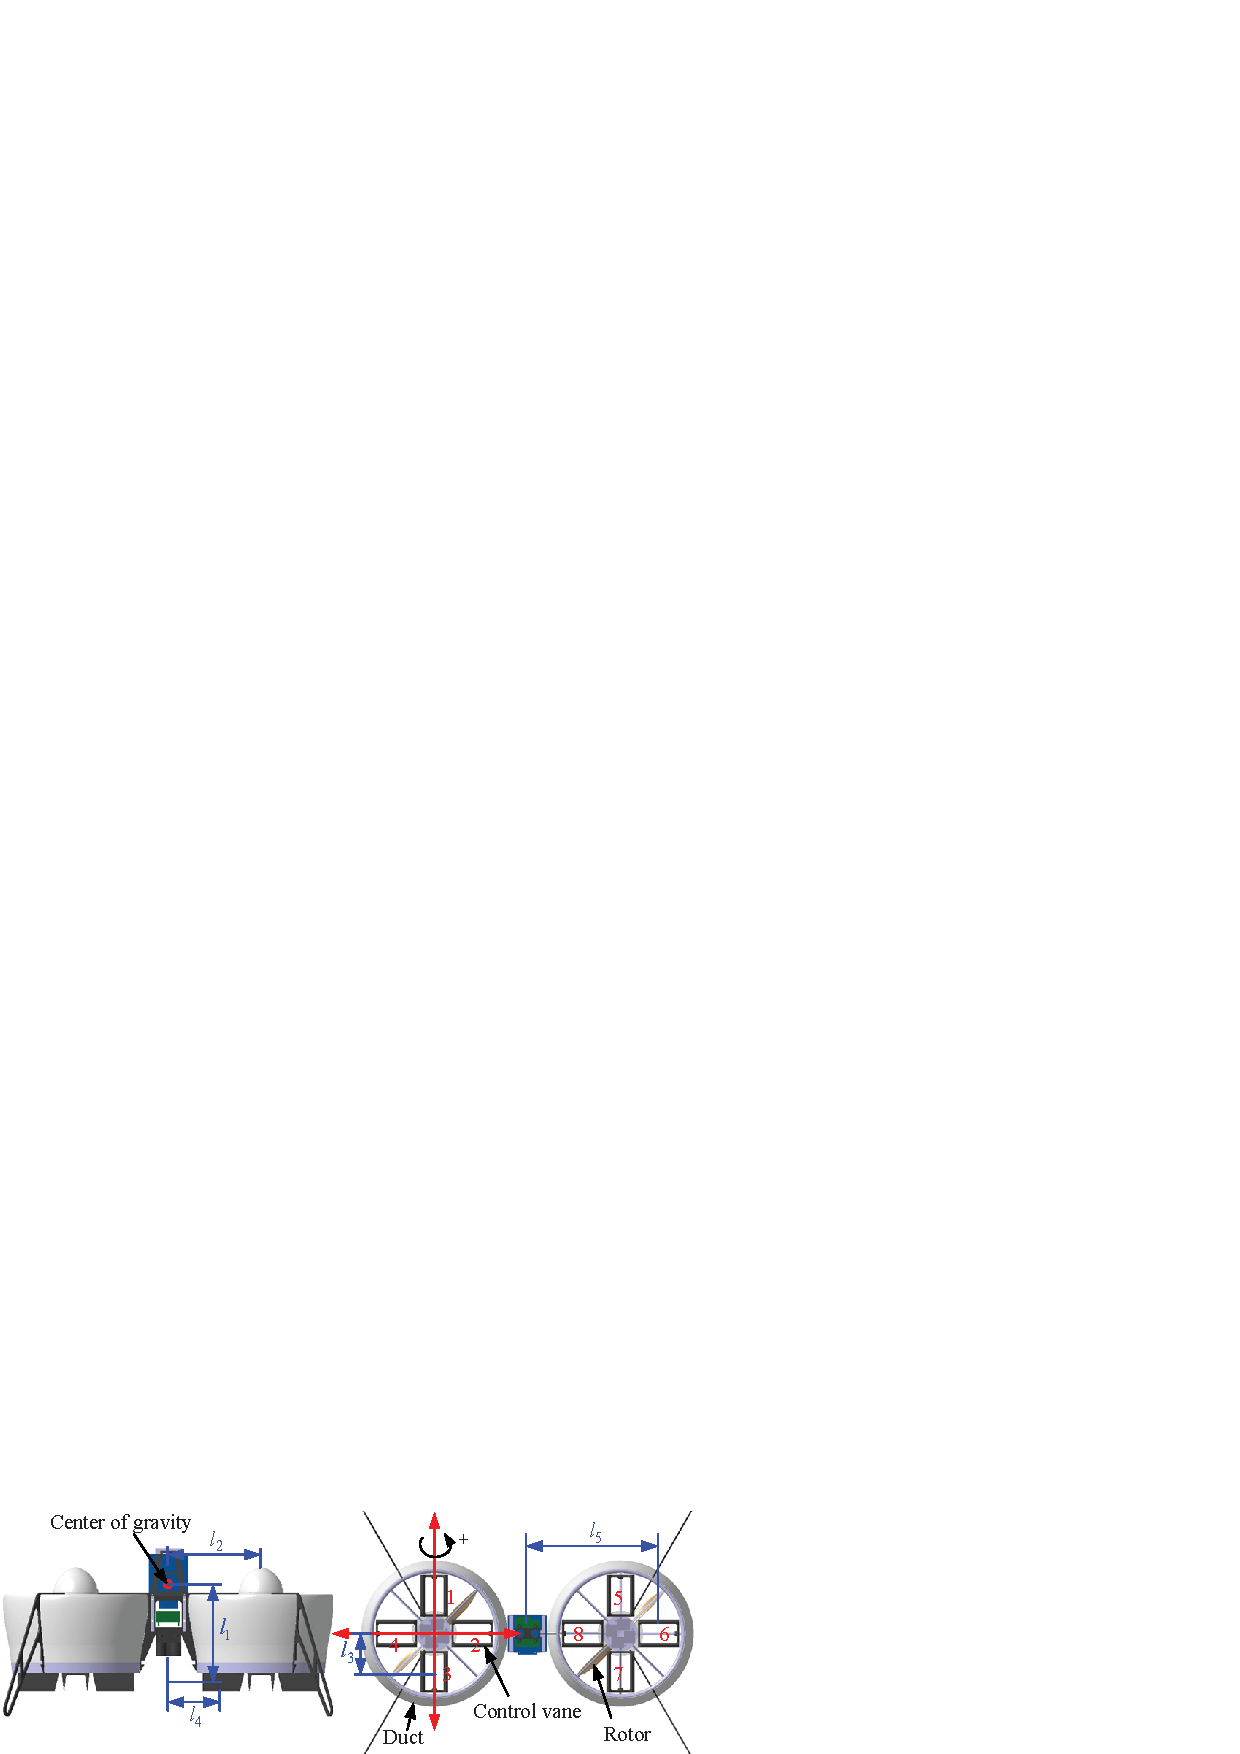
\includegraphics[scale=1]{Fig/Fig2.pdf}}
%		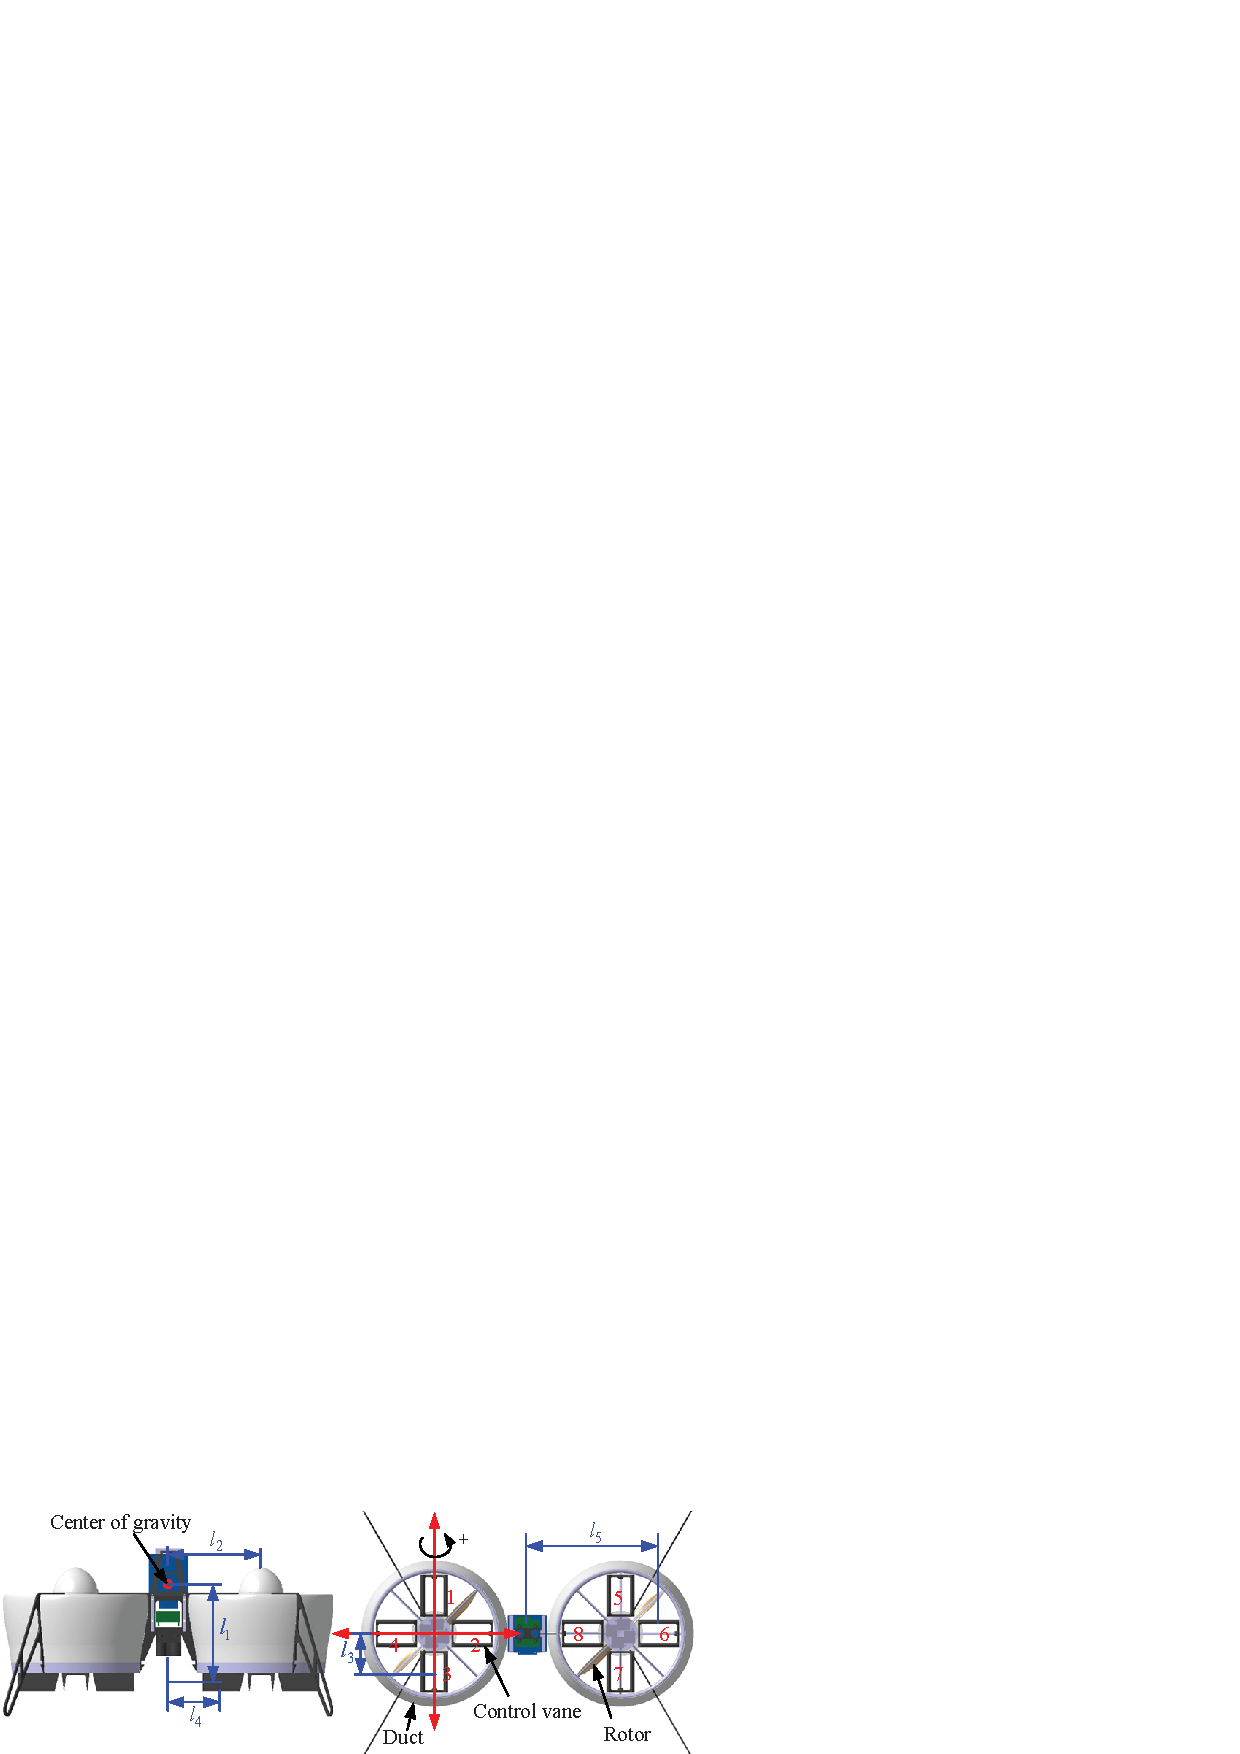
\includegraphics[scale=1]{Fig/Fig2.pdf}
%	\end{minipage}%
%	\begin{minipage}[c]{0.55\textwidth}
%		\centering
%%		\fbox{\includegraphics[scale=1.2]{Fig/Fig3.pdf}}
%		\includegraphics[scale=1.2]{Fig/Fig3.pdf}
%	\end{minipage}\\[1pt]
%	\begin{minipage}[t]{.45\textwidth}
%		\caption{\label{fig_euler}欧拉角及坐标系定义}
%	\end{minipage}%
%	\begin{minipage}[t]{.55\textwidth}
%		\caption{\label{arm}力臂示意图}
%	\end{minipage}%
%\end{figure}
定义操纵面旋转轴如图\ref{DFUAV_arm}所示,其中1号、2号操纵面旋转轴分别和机体系$ \bm{X}_b $轴和$ \bm{Y}_b $轴方向相同,1、3号操纵面产生滚转力矩,2、4号操纵面产生俯仰力矩。所有操纵面用于产生偏航力矩。规定操纵面旋转符合右手系则操纵面偏转角$\delta_i  $,$ i=1,2,3,4 $为正值,否则为负值。零偏转定义在操纵面平行于${{\bm{Z}}_{B}}$轴的位置。每个操纵面最大转动角度均为$\pm {{20}^{{}^\circ }}$。力臂${{l}_{1}}$、${{l}_{2}}$如图\ref{DFUAV_arm}所示。则每个操纵面上产生的升力可表示为\cite{Wu_2011,Zhao_2015,Graf_2008}
\begin{align}\begin{array}{l}
%F_{i}=\dfrac{1}{2} \rho S_{v} (V_i+V_c)^{2} C_{v} 
F_{i}=  k_{\delta} (V_i+V_c)^{2} \delta_{i} 
\end{array}	\label{F_i}
\end{align}
%\begin{align}\begin{array}{l}
%D_{\delta i}=  k_{D} F_{i}^{2}
%\end{array}\end{align}
其中$  k_{\delta} $为操纵面气动升力系数,和攻角$ \alpha_d $有关,$ V_i+V_c $为涵道出口气流流速。由操纵面产生的作用于机体的力和力矩可分别表示为\cite{Pflimlin_2007a}
\begin{align}
\bm{F}_{c}=\begin{bmatrix}
F_4-F_2	\\
F_1-F_3 \\
0
%D_{\delta 1}+D_{\delta 2}+D_{\delta 3}+D_{\delta 4}
\end{bmatrix}
\end{align}
\begin{align}\bm{M}_{c}=
\begin{bmatrix}
\tau_{x } \\
\tau_{y } \\
\tau_{z }
\end{bmatrix}
=
\begin{bmatrix}
-{{l}_{1}}\left(F_{1}-F_{3}\right) \\
{{l}_{1}}\left(F_{4}-F_{2}\right) \\
{{l}_{2}}\left(F_{1}+F_{2}+F_{3}+F_{4}\right)
\end{bmatrix}	\label{eq_M_c}
\end{align}
其中$ \bm{M}_{c} $又称驱动力矩,$ \tau_{x } $、$ \tau_{y } $、$ \tau_{z } $为驱动力矩在机体系坐标轴上的投影。在下一章控制系统设计中,控制律将给出期望的驱动力矩。
%\begin{align}
%%V_{e}=\frac{V_{0} \cos \alpha+\sqrt{\left(V_{0} \cos \alpha\right)^{2}+\frac{4 F_{t}}{\rho A_{d}}}}{2} \\
%C_{v}=C_{\delta}\left(\delta_{i}+\delta_{0}+\delta_{p}\right)
%\end{align}
%其中$ \rho $为流体密度,$ S_{v} $为操纵面面积,$ V_i+V_c $为涵道出口气流流速,$ C_{v} $为升力系数,$ C_{\delta} $为升力系数的斜率,$ \delta_{i} $、$ \delta_{0} $分别为操纵面偏转角和操纵面翼型的零升力偏转角度。当无人机向前飞行时,操纵面同时处于涵道风扇的尾流和前向飞行来流中。 合成气流方向和涵道的机体系$ z $轴成一个偏斜角$ \delta_{p} $,可表示为\cite{Tobias_2008a}
%\begin{align}\delta_{p}=\arctan \frac{\eta V_b \sin \alpha_d}{v_b+w \cos \alpha_d}\end{align}

%其中$\bm{\delta}$
% $k_{\delta}$为操纵面气动力系数, $V_d$为涵道底部吹出的气流速度。
%由于控制表面是可移动的平板提升表面,因此它们产生的提升力将取决于它们的有效攻角。 迎角是控制表面挠度,局部气流速度和由导管引起的向下冲洗的函数。 由于控制面的位置远离重心,因此包含了一些术语以说明由于车辆的角速度而引起的气流。 以下表达式指定这些影响如何影响升力,副翼和舵的迎角:
%\begin{align}\begin{array}{c}
%\alpha_{e}=\delta_{e}+\tan ^{-1}\left(-v_{x}-\omega_{y} l_{e}, v_{i}-v_{z}\right)-\gamma_{x} \\
%\alpha_{a}=-\delta_{a}+\tan ^{-1}\left(-v_{y}+\omega_{x} l_{a}, v_{i}-v_{z}\right)-\gamma_{y} \\
%\alpha_{r}=\delta_{r}+\tan ^{-1}\left(-\omega_{z} l_{r}, v_{i}-v_{z}\right)
%\end{array}\end{align}
%在这些表达式中,$ \delta $项表示控制面的挠度,而$ l $项表示控制面的空气动力学中心与车辆重心之间的距离。 术语“升降机”,“副翼”和“方向舵”在直升机模式下应用于控制面。 因此,舵表示风管流出的叶片,升降舵和副翼是位于机身末端的控制面。
%
%类似地,可以通过为每个控制面包括适当的速度分量来找到每个控制面所经历的动压力的表达式:
%\begin{align}\begin{array}{c}
%q_{e}=\dfrac{1}{2} \rho_{\infty}\left[\left(v_{i}-v_{z}\right)^{2}+\left(v_{x}+\omega_{y} l_{e}\right)^{2}\right] \\
%q_{a}=\dfrac{1}{2} \rho_{\infty}\left[\left(v_{i}-v_{z}\right)^{2}+\left(v_{y}-\omega_{x} l_{a}\right)^{2}\right] \\
%q_{r}=\dfrac{1}{2} \rho_{\infty}\left[\left(v_{i}-v_{z}\right)^{2}+\left(\omega_{z} l_{r}\right)^{2}\right]  \label{dynamic_pressure}
%\end{array}
%\end{align}
%
%使用式\eqref{dynamic_pressure}具有用于各种控制表面的适当参数,基于控制表面迎角提供了控制表面升力系数。这使我们能够找到与车身轴线垂直的提升力分量以及这些力产生的力矩。
%\begin{align}
%\begin{array}{c}
%\bm{F}_{\mathrm{cs}}=\left[\begin{array}{c}
%\operatorname{sgn}\left(v_{i}-v_{z}\right) C_{L, e} q_{e} \cos \left(\alpha_{e}-\delta_{e}\right) S_{e} \\
%\operatorname{sgn}\left(v_{i}-v_{z}\right) C_{L, a} q_{a} \cos \left(\alpha_{a}+\delta_{a}\right) S_{a} \\
%0
%\end{array}\right] \\
%\bm{M}_{\mathrm{cs}}=\left[\begin{array}{c}
%-\operatorname{sgn}\left(v_{i}-v_{z}\right) C_{L, a} q_{a} \cos \left(\alpha_{a}+\delta_{a}\right) S_{a} l_{a} \\
%\operatorname{sgn}\left(v_{i}-v_{z}\right) C_{L, e} q_{e} \cos \left(\alpha_{e}-\delta_{e}\right) S_{e} l_{e} \\
%\operatorname{sgn}\left(v_{i}-v_{z}\right) C_{L, r} q_{r} \cos \left(\alpha_{r}-\delta_{r}\right) S_{r} l_{r}
%\end{array}\right]
%\end{array}\end{align}
%S项代表每个控制表面的总面积。 请注意,对于操纵面,阻力和力矩的影响已被忽略。
\subsection{固定气动面动力学和陀螺力矩}
单涵道无人机内部设计固定气动面以平衡悬停状态下风扇反扭距的影响。如图\ref{F_af}所示,
%单个固定气动面上的力$ F_af $为:
%\begin{align}
%F_{a f}=\int d F \\
%d F=\frac{1}{2} \rho c_{a f} V_{a f}^{2} C_{L a f} \cdot d R
%\end{align}
%其中$ c_af $为单个气动面的弦长,$ R $为半径,$ V_{af} (R)=√((ω_w R)^2+(V_c+V_i )^2 ) $为入流速度,$ C_{Laf}=C_{laf} \alpha_{af} $为气动面的升力系数,$ C_{laf} $为翼型的升力线斜率,$ \alpha_{af} $为入流的有效迎角,满足:
%\begin{align}
%\alpha_{a f}=\varphi_{b}+\varphi_{0}
%\end{align}
%其中,$ φ_b $为旋转流场的入流角,
固定气动面对涵道轴的力矩可近似为:
\begin{align}\bm{M}_{a f}=\left(V_{c}+V_{i}\right)^{2} \varphi_{0}\left[\begin{array}{c}
0 \\
0 \\
d_{a f}
\end{array}\right]+\left(V_{c}+V_{i}\right) \varpi \left[\begin{array}{c}
0 \\
0 \\
d_{d s}
\end{array}\right]	\label{M_af}
\end{align}
其中$ d_{af} $ 、$ d_{ds} $为常系数,$ \varphi_0 $为气动面安装角。
\begin{figure}[htbp]
	\centering
	\includegraphics[scale=1]{Fig/F_af1.pdf}
	\caption{\label{F_af}固定气动面上的流场及气动力}
\end{figure}

在悬停点附近,涵道风扇转速几乎恒定,只有在剧烈的机动飞行中,转速变化才会比较明显。 为简单起见,假设风扇转速的变化可以忽略不计。 因此,由风扇的旋转产生陀螺力矩可表示为
\begin{align}
\bm{M}_{{g}}=-\bm{\omega} \times \bm{L}_{{r}}=b I_{b} \varpi
\begin{bmatrix}
-q \\
p \\
0
\end{bmatrix}
\end{align}
其中$ I_{b} $为风扇转动惯量,$ \bm{L}_{{r}} $为风扇角动量。
\section{双涵道动力学分析}
在悬停工作点附近,双涵道的动力学模型可以由单涵道推广而来,其左侧涵道和上述单涵道类似,右侧涵道是左侧的镜像,即风扇反向旋转且固定气动面反向安装。在双涵道中,总的气动力$ \bm{F} $是左右两个涵道所受气动力的矢量和,记为
\begin{align}
\bm{F}&=\bm{F}_{L}+\bm{F}_{R}
\end{align}
其中$ \bm{F}_{L} $为左边涵道所受气动力,$ \bm{F}_{R} $为右边涵道所受气动力。其表达式和单涵道类似,以$ \bm{F}_{L} $为例,可以表示为
\begin{align}
\bm{F}_{L} &=\bm{F}_{La}+\bm{F}_{Lr}+\bm{F}_{Ld}+\bm{F}_{Lc} 
\end{align}
$ \bm{F}_{R} $的表达式完全类似。类似的,总的气动力矩力矩$ \bm{M} $可表示为
\begin{align}
\bm{M}&=\bm{M}_{L}+\bm{M}_{R}
\end{align}
其中$ \bm{M}_{L} $为左边涵道所受气动力矩,$ \bm{M}_{R} $为右边涵道所受气动力矩。以左侧涵道为例,由力和力矩的关系,气动力矩可表示为
\begin{align}
\bm{M}_{L} &=\bm{l} \times \bm{F}_{L}  
\end{align}
其中矢量$ \bm{l} $力的作用点在机体系的坐标表示。本节仅讨论和本文主题相关双涵道操纵面动力学部分,详细的双涵道建模可参考\cite{Speck_2013,Speck_2013a}。
%\subsection{机身动力学}
%机身空气阻力产生的力可以写为:
%\begin{align}
%\bm{F}_{{a}} = \bm{F}_{{La}}+\bm{F}_{{Ra}}
%\end{align}
%其中$ \bm{F}_{{La}} $、$ \bm{F}_{{Ra}} $的表达式由式\eqref{eq_F_a}确定。对应的力矩为
%\begin{align}
%\bm{M}_{{a}} = \bm{M}_{{La}}+\bm{F}_{{Ma}}= \bm{l}_{aL} \times \bm{F}_{{La}}+ \bm{l}_{Ra} \times \bm{F}_{{Ra}}
%\end{align}
%其中$ \bm{l}_{aL} $、$ \bm{l}_{aR} $分别代表左、右侧涵道的机身气动力作用点在机体系的坐标表示。。
\subsection{涵道风扇动力学}
作用于无人机的推力
\begin{align}
\bm{F}_{r}=\bm{F}_{{Lr}}+\bm{F}_{{Rr}}=\begin{bmatrix}
0\\0\\
-T_{La}-T_{Ra}
\end{bmatrix}
\end{align}
其中$ T_{{La}} $、$ T_{{Ra}} $的表达式由上一节求解$ T_a $的方法确定。考虑到风扇上的升力差会产生一个滚转力矩,因此风扇产生的扭矩可表示为
\begin{align}
\bm{M}_{r}=\begin{bmatrix}
(T_{La}-T_{Ra})l_2\\0\\
Q_{L}-Q_{R}
\end{bmatrix}	\label{eq_prop}
\end{align}
其中$ Q_{R} $前的负号是由于右边的风扇是顺时针转动的,$ l_2 $为两个涵道风扇的旋转中心的距离,$ Q_{L}$、$Q_{R} $类似的由式\eqref{eq_Q}确定。
%\subsection{涵道动力学}
%左右两侧的动量阻力完全类似,总的动量阻力表示为
%\begin{align}
%\bm{F}_{m}=\bm{F}_{{Lm}}+\bm{F}_{{Rm}}
%\end{align}
%测风产生的力矩为
%\begin{align}
%\bm{M}_{{l}}=\bm{l}_{Lm} \times \bm{F}_{{Lm}}+\bm{l}_{Rm} \times \bm{F}_{{Rm}}
%\end{align}
%其中$ \bm{l}_{Lm} $、$ \bm{l}_{Rm} $为力臂矢量。
%
%参照上一节,涵道产生的力和力矩可分别表示为
%\begin{align}
%\bm{F}_{{d}}=
%\begin{bmatrix}
%L_{Lx}+L_{Rx}+D_{Lx}+D_{Rx} \\
%L_{Ly}+L_{Ry}+D_{Ly}+D_{Ry} \\
%L_{Lz}+L_{Rz}+D_{Lz}+D_{Rz}
%\end{bmatrix}
%+\bm{F}_{{m}} 
%\end{align}
%\begin{align}
%\bm{M}_{{d}}=
%\begin{bmatrix}
%(L_{Lx}+L_{Rx}) l_{d} \\
%(L_{Ly}+L_{Ry}) l_{d} \\
%0
%\end{bmatrix}
%+\bm{M}_{{l}}
%\end{align} 
\subsection{操纵面动力学}
类似单涵道,定义操纵面旋转轴如图\ref{TDFUAV_arm}所示,其中1号、2号操纵面旋转轴分别和机体系$ \bm{X}_b $轴和$ \bm{Y}_b $轴方向相同,1、3、5和7号操纵面产生滚转力矩,2、4、6和8号操纵面产生俯仰力矩。所有操纵面用于产生偏航力矩。零偏转定义在操纵面平行于${{\bm{Z}}_{B}}$轴的位置。操纵面偏转角$\delta_i  $,$ i=1,2,\ldots,8 $最大转动角度均为$\pm {{20}^{{}^\circ }}$。力臂如图\ref{DFUAV_arm}所示。每个操纵面上的升力$ F_i $由式\eqref{F_i}给出,为简单起见,忽略操纵面阻力,则操纵面气动力和驱动力矩可表示为
\begin{figure}[htbp]
	\centering	
	\includegraphics[scale=1]{Fig/TDFUAV_arm.pdf}%
	\caption{\label{TDFUAV_arm}双涵道力臂示意图}
\end{figure}
\begin{align}
\bm{F}_{c}=\begin{bmatrix}
-F_2+F_4-F_6+F_8	\\
F_1-F_3+F_5-F_7 \\
0
%D_{\delta 1}+D_{\delta 2}+D_{\delta 3}+D_{\delta 4}
\end{bmatrix}
\end{align}
\begin{align}\bm{M}_{c}=
\begin{bmatrix}
\tau_{x } \\
\tau_{y } \\
\tau_{z }
\end{bmatrix}
=
\begin{bmatrix}
-{{l}_{1}}\left(F_1-F_3+F_5-F_7\right) \\
{{l}_{1}}\left(-F_2+F_4-F_6+F_8\right) \\
\left(l_3 F_{1} - l_4 F_{2} + l_3 F_{3} + l_5 F_{4} + l_3 F_5 + l_5 F_6 + l_3 F_7 + -l_4 F_8 \right)
\end{bmatrix}	\label{eq_TDF_M_c}
\end{align}	
%\subsection{固定气动面动力学和陀螺力矩}
%双涵道内部的固定气动面完全类似单涵道,并且左右两边互为镜像,即旋翼(风扇)转动方向相反,固定气动面安装方向相反。双涵道固定气动面对涵道轴的力矩可表示为:
%\begin{align}
%\bm{M}_{a f}=\bm{M}_{Laf}+\bm{M}_{Raf}
%\end{align}
%其中$ \bm{M}_{Laf} $ 、$\bm{M}_{Raf} $分别与左右两侧涵道的旋翼转速相关,由式\eqref{M_af}确定。旋翼的旋转产生陀螺力矩表示为
%\begin{align}
%\bm{M}_{{g}}=-\bm{\omega} \times (\bm{L}_{{Lr}}-\bm{L}_{{Rr}})=b (I_{Lb}\varpi_L-I_{Rb}\varpi_R)
%\begin{bmatrix}
%-q \\
%p \\
%0
%\end{bmatrix}
%\end{align}
%其中$ I_{Lb} $、$ I_{Rb} $为左右两侧旋翼转动惯量,$ \varpi_L $、$ \varpi_R $为左右两侧旋翼转速。
\section{涵道无人机仿真模型}
利用CDF计算得涵道模型参数如表\ref{DF_para}、表\ref{TDF_para}所示,其中表\ref{TDF_para}仅列出和单涵道不同的参数。将上述与力和力矩有关的方程用借助MATLAB$^\circledR$/Simulink$^\circledR$的S-函数实现,式\eqref{eq_nonlinear_model}用Simulink$^\circledR$库自带的六自由度刚体模块实现,被控对象的仿真图如图\ref{fig_plant_simulink}所示。其中“Actuators”表示操纵面偏转角$ \bm{\delta} $信号输入,“Environment”表示状态反馈和环境变量(重力,风扰等)。“Calculate Force”表示计算作用于无人机的力,“Calculate Torque”表示计算作用于无人机的力矩,这两个模块内部分别如图\ref{fig_force_simulink}、图\ref{fig_moment_simulink}所示,其中$\mathrm{R}^{\wedge} \mathrm{T}$ 表示$ R^T $,“$ \mathrm{s\_{}Force} $”是计算作用于无人机的气动力的S-函数,“$ \mathrm{s\_{}Torque} $”是计算作用于无人机的气动力矩的S-函数。

\begin{table}
\caption{\label{DF_para}单涵道模型参数}
	\centering{}%
	\small 
	\begin{tabular}{cccccc}
		\hline 
		参数符号 & 数值&参数符号 & 数值&参数符号 & 数值\tabularnewline
		\hline 
		$ A_x,A_y,A_z $  & $ 0.04082\,\text{m}^2 $ &$ \rho $        &$1.225\,\text{kg}/\text{m}^3$&$ I_b $           & $ 0.000029 $               \tabularnewline
		$ k_{\varpi} $   & $1.13342 \times 10^{-6}$& $ d_{\varpi} $ & $1.13342 \times 10^{-7}$ 	  &$k_{\delta} $     & $ 0.01495 $ 			      \tabularnewline
		$C_{D,x},C_{D,y}$& $ 0.43213 $             &$ C_{D,z} $     & $ 0.13421 $             	  &	$ q_a $ 	     & $ 1.49 $ 				  \tabularnewline
	    $ l_{a} $        & $ -0.1121\,\text{m} $   & $ d_{ds} $     & $ 0.01495 $			  	  &$ d_{af} $        & $ 0.01495 $    			  \tabularnewline
		$ R $            & $ 0.11\,\text{m} $      &$ b $           & $ 2 $       			   	  &$ S $ 			 & $ 0.04082\,\text{m}^2 $    \tabularnewline
		$C_{l_{\alpha}}$ & $ 2.212\,/\text{rad} $  &$C_{l, \max } $ & $ 1.05 $ 				   	  &$ C_{l, \min } $  & $ -1.05 $ 				  \tabularnewline
		$ l_2 $          & $ 0.06647\,\text{m} $   &$ l_1 $         & $ 0.17078\,\text{m} $    	  &	$ m $ 		     & $ 1.53\,\text{kg} $ 		  \tabularnewline
		$ C_{d, o } $    & $ 0.9 $                 &$ C_{d, g } $   & $ 0.9 $					  &$ C_{duct} $      & $ 0.78497 $	 			  \tabularnewline
		$ I_x $          & $ 0.02548 $ 			   &$ I_y $         & $ 0.02550 $                 &$ I_z $			 & $ 0.00562 $ 				  \tabularnewline
		\hline 
	\end{tabular}	
\end{table}

\begin{table}
	\caption{\label{TDF_para}双涵道模型参数}
	\centering{}%
	\small 
%	\resizebox{\textwidth}{!}{
	\begin{tabular}{cccccc}
		\hline 
		参数符号 & 数值&参数符号 & 数值&参数符号 & 数值\tabularnewline
		\hline 
		$ I_x $ & $ 054593 $ &$ I_y $ & $ 0.017045 $& $ I_z$ & $ 0.049226 $ \tabularnewline
	    $ l_{1} $ & $ 0.0808\,\text{m} $&$ l_{2} $ & $ 0.175\,\text{m} $ &$ l_3 $ & $ 0.06647\,\text{m} $ \tabularnewline 
		$ l_4 $ & $ 0.2415\,\text{m} $ &$ l_5 $ & $ 0.1085\,\text{m} $& $ m $ & $ 3.7\,\text{kg} $ \tabularnewline
		\hline 
	\end{tabular}	%}
\end{table}
\begin{figure}[htbp]
	\centering
	\includegraphics[scale=0.35]{Fig/Fig_model.png}
	\caption{\label{fig_plant_simulink}被控对象simulink}
\end{figure}
\begin{figure}[htbp]
	\centering
	\includegraphics[scale=0.3]{Fig/Fig_Force.png}
	\caption{\label{fig_force_simulink}Calculate Force模块}
\end{figure}
\begin{figure}[htbp]
	\centering
	\includegraphics[scale=0.32]{Fig/Fig_Torque.png}
	\caption{\label{fig_moment_simulink}Calculate Torque模块}
\end{figure}
\section{本章小结}
本章建立了涵道风扇式无人机的数学模型。首先对无人机的运动进行参数化,定义了坐标系。然后推导了运动方程,再对运动方程中涉及的气动力和气动力矩进行分析。最后根据所建立的模型建立MATLAB$^\circledR$/Simulink$^\circledR$仿真,仿真中将该模块作为被控对象,然后针对该对象设计控制器以及分配器。





%\subsection{旋翼模型}
%旋翼模型基于基本动量理论和叶片元素理论进行推导的,这里的推导类似直升机的旋翼模型的推导,虽然并不能解决管道中的不稳定气流的建模问题,但有证据表明这种模型确实提供了对旋翼性能的足够准确的刻画\cite{Johnson_2005}。经过旋翼的气流流速受沿机体$ z $轴的速度$ w$以及旋翼叶片的转速和旋翼叶片的几何形状影响,可表示为\cite{Heffley_1988}
%\begin{align}
%V_i+V_c=w+\dfrac{2}{3} \varpi r\left(\dfrac{3}{4} K_{t w i s t}\right)
%\end{align}
%其中$ \varpi $代表旋翼转速,$ r $是旋翼半径,而$ K_{t w i s t} $是叶片的扭转。 推力现在可以写成\cite{Heffley_1988}
%\begin{align}
%F_T=\dfrac{1}{4}\left(V_i+V_c-v_{i}\right) \varpi r^{2} \rho_{\infty} a_{0} b c_{r}
%\end{align}
%其中,$ v_{i} $表示通过旋翼处气流的的诱导速度,$ a_{0} $表示旋翼升力曲线斜率,$ b $表示旋翼的叶片数,$ c_{r} $是旋翼叶片的弦长。 涵道远端的气流速度可以表示为\cite{Stepniewski_2013}
%\begin{align}
%v^{\prime}=\sqrt{u^{2}+v^{2}+\left(w-v_{i}\right)^{2}}
%\end{align}
%现在可以将诱导速度表示为\cite{Stepniewski_2013}
%\begin{align}
%v_{i}=\dfrac{F_T}{2 \rho_{\infty} \pi r^{2} v^{\prime}}
%\end{align}
%这些方程是迭代求解的。 综上,作用在无人机上的旋翼产生的推力可以表示为
%\begin{align}
%\bm{F}_{r}=\begin{bmatrix}
%0\\0\\
%-F_T
%\end{bmatrix}
%\end{align}
%
%施加在旋翼上的反扭矩表达式需要功率来计算。 诱导功率和翼型功率为\cite{Heffley_1988}
%\begin{gather}
%P_{i}=\tau\left(v_{i}-w\right) \\
%P_{p}=\dfrac{1}{8} \rho_{\infty} f_{r} r \varpi\left[\left(r \varpi\right)^{2}+4.6\left(u^{2}+v^{2}\right)\right]
%\end{gather}
%$ f_{r} $代表旋翼摩擦项,有\cite{Heffley_1988}
%\begin{align}
%f_{r}=C_{D_{o}} r b c_{r_{r}}
%\end{align}
%空气施加在旋翼上的力矩可以表示为\cite{Johnson_2005}
%\begin{align}M_{r}=\dfrac{P_{i}+P_{p}}{\omega_{r}}\end{align}
%发动机功率与旋翼转速和油门位置的关系可表示为\cite{Johnson_2005}
%\begin{align}
%P_{e}=\dfrac{x_{thr} K_{b} \eta_{e} \min \left(\varpi K_{d}, K_{r }\right)}{K_{r }}
%\end{align}
%其中$ x_{t}  $表示油门位置,$ K_{b} $是发动机的马力,$ \eta_{e} $是发动机效率,$ K_{d} $是主风扇齿轮比,而$ K_{r} $是发动机每秒的最大转数。 控制油门状态的微分方程为
%\begin{align}
%\dot{x}_{t}=\dfrac{\delta_{t}-x_{t}}{K_{t}}
%\end{align}
%其中$ \delta_{t} $表示油门输入,$ K_{t} $是发动机时间常数。 从顶部看时旋翼是逆时针旋转的,发动机施加的力矩可表示为
%\begin{align}
%M_{e}=\dfrac{P_{e}}{\varpi K_{d}} 
%\end{align}
%\begin{gather}
%\bm{M}_{{r}}=\begin{bmatrix}
%0 \\
%0 \\
%M_{e} K_{d}
%\end{bmatrix}	\label{M_rotor}
%\end{gather}
%最后,控制风扇转速的微分方程为
%\begin{align}
%\dot{\bar{\omega}}_{r}=\dfrac{M_{e} K_{d}-M_{r}}{b i_{b}}
%\end{align}
%其中$ i_{b} $表示单个叶片绕旋转轴的惯性矩。












